\subsection{Método propuesto}
Como alternativa para mejorar la medidas de comparación entre datos de texto en sitios de CQA bajo una arquitectura Big Data se propone en este trabajo el método EQuAL (\textit{Ensemble method for community Question Answering sites based on cLustering}), basado en un método de ensamble de clustering de acumulación de evidencias, que puede ser utilizado para la generación de matrices de similaridad que sirven como entrada para un RS en un sitio de CQA. Este método está basado en una arquitectura Big Data distribuida y tiene en cuenta diversas distancias de texto, combinadas mediante un método de ensamble de clustering.

\begin{figure}[h!]
	\centering
	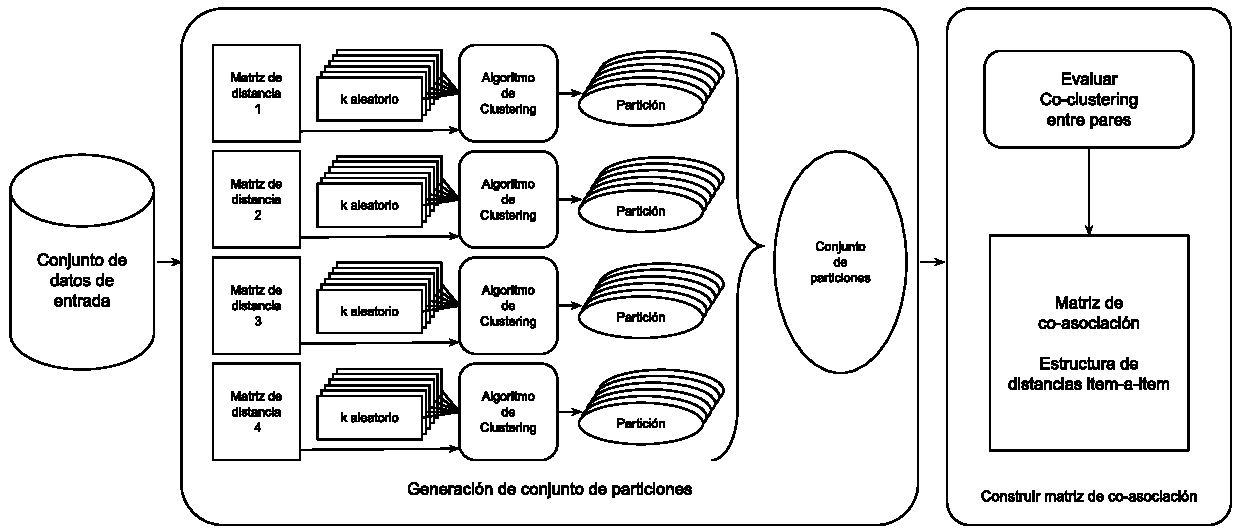
\includegraphics[width=0.9\linewidth]{8_problema_investigacion/imagenes/metodo_equal}
	\caption{Método EQuAL para la generación de matrices de co-asociación desde el conjunto de datos original.}
	\label{fig:metodoequal}
\end{figure}

El desarrollo para este método está basado en dos pasos: \begin{enumerate*} [label=(\roman*)] \item la generación de conjunto de particiones y \item la construcción de matriz de co-asociación. \end{enumerate*} La Figura \ref{fig:metodoequal} muestra un ejemplo del método, en el cual la primera etapa está compuesta de 4 matrices de distancias procesadas a través de un algoritmo de clustering, formando un conjunto de particiones, para luego, en la segunda etapa, ser ensambladas para formar la matriz de co-asociación. Veremos este proceso en detalle a continuación.


\subsubsection{Generación de conjunto de particiones}
El primer paso es la generación de un conjunto de particiones. El procedimiento comienza aplicando los distintos algoritmos de medidas de similaridad de texto del estado del arte al conjunto de datos de entrada. Por cada algoritmo, este procedimiento tiene como resultado una matriz de similaridad. Cada una de las matrices de similaridad es el resultado de la combinación de todas las preguntas (individuales) de un muestreo original.

\bigskip Por cada matriz de similaridad, se aplican \(c\) corridas de algoritmos de clustering, cada uno con un número \(k\) de elementos seleccionados al azar\footnote{Recordar de la Sección \ref{sec:clustering} que el número \(k\) es un parámetro de entrada del algoritmo de clustering que representa el número de clusters que se generarán.}. Esta combinación de \(n\) matrices y \(c\) ejecuciones del proceso de clustering, resulta en \(N = n \times c\) salidas del algoritmo de clustering elegido como resultado. Cada salida consiste en una partición\footnote{Recordar de la Sección \ref{sec:algoritmos_clustering} el concepto de partición en el contexto de clustering.} \(P\) donde cada elemento consiste en la asignación de una pregunta individual a un cluster específico.

\bigskip Con el fin de resumir la estructura de todas las particiones generadas por los algoritmos de clustering, se unen las particiones anteriormente obtenidas, dando lugar a un conjunto de particiones \(\rm I\!P\) de la siguiente manera:
\[\rm I\!P = \{P^1, P^2, ..., P^N\},\]
donde \(N\) es el número de particiones que conforman el conjunto que será la entrada del procedimiento de construcción de la matriz de co-asociación.

\subsubsection{Construcción de la matriz de co-asociación}
El segundo paso es construir una matriz de co-asociación a partir del conjunto de particiones \(\rm I\!P\). Para tal fin, se aplica un algoritmo de ensamble de clustering de acumulación de evidencias, que combina cada una de estas particiones, dando como salida una matriz de co-asociación. Cada valor \(i,j\) perteneciente a la matriz de co-asociación consiste en la proporción de veces que los elementos \(i,j\) caen juntos en el mismo grupo de la salida de clustering, a lo largo de las \(N=n \times c\) particiones.

\bigskip La matriz de co-asociación, que es una representación integrada de las relaciones subyacentes entre los datos originales, es la entrada propuesta como nueva medida de distancia para datos de texto en sitios CQA para construir RS. Esta medida tiene la característica de ser adimensional, ya que consiste en una proporción respecto del total de datos, y además considera toda la variabilidad propia de los algoritmos de clustering utilizados para su construcción, por lo cual toma en cuenta la estructura de distancia ítem-ítem que es necesaria como entrada para un RS basado en contenido incorporando varios aspectos de las distancias entre elementos de texto, en lugar de usar solo una simple medida basada individualmente en aspectos de cada una de las medidas de distancia.

\bigskip El armado de matrices, la combinación de las mismas y la aplicación de estrategias para su procesamiento, implica un aumento significativo del volumen de datos y requiere una capacidad de cálculo intensiva. Una arquitectura Big Data que realice el procesamiento distribuido de los mismos es fundamental para este proceso. Además del volumen de datos con el cual se trabajará, se varían distintos parámetros, tales como la medida de similaridad y valores de umbral involucrados en procesos de clustering, con el fin de obtener resultados confiables. Esta característica redunda en múltiples ejecuciones de toda la solución. En pos de lograr una solución eficiente, cabe destacar que se implementaron experimentos basados en una infraestructura MapReduce aplicados con frameworks basados en Hadoop y cluster computing, lo cual provee la ventaja de procesar grandes cantidades de datos en instancias dinámicamente escalables, logrando cumplir con los preceptos de velocidad, variedad y veracidad del Big Data.